% LNCS paper, based on samplepaper.tex
\documentclass[runningheads]{llncs}
\usepackage[T1]{fontenc}
\usepackage{graphicx}
\usepackage{booktabs}
\usepackage{tabularx}
\usepackage{array}
\usepackage{amsmath}
\usepackage[section]{placeins}
\newif\ifanonymous
%\anonymoustrue      % wersja do double blind review
\anonymousfalse   % wersja camera-ready
\begin{document}
\title{Prediction or Revaluation? Phase- and Space-Aware VAEP for Women's Football}
\titlerunning{Phase-Space VAEP for Women's Football}
\ifanonymous
  \author{Anonymous Author(s)}
  \authorrunning{Anonymous Author(s)}
  \institute{Paper under double-blind review}
\else
\author{
Tomasz Piłka\inst{1}\orcidID{0000-0003-1206-2076} \and
Kaj Skubiszak\inst{2}\orcidID{0009-0003-9004-4620} \and
Piotr Andrzejewski\inst{3}\orcidID{0009-0001-3721-6046} \and
Patryk Żyliński\inst{4}\orcidID{0009-0002-2119-5292}
}
\authorrunning{T. Piłka et al.}
\institute{Faculty of Mathematics and Computer Science, \\Adam Mickiewicz University in Pozna\'n, Poland \\
\email{tomasz.pilka@amu.edu.pl} \\
\email{\{kajsku, pioand6, patzyl\}@st.amu.edu.pl}}
\fi
\maketitle
\begin{abstract}
Event-based action valuation models, such as VAEP, assign value to on-ball actions based on their type, outcome, location, and recent context, but they do not encode the off-ball spatial configuration in which the action is performed. This limitation is particularly relevant in women's football, where public spatial data remains scarce. We study whether two interpretable context layers, rule-based tactical phase labels and geometric features from StatsBomb 360 freeze frames, affect VAEP-style action valuation in a men-to-women source-target learning setting.
We compare three nested variants: Event-VAEP, Phase-VAEP and Phase-Space VAEP. The models are evaluated on a held-out women's tournament in terms of discrimination, calibration, source-target training strategy and player valuation behaviour, with paired match-level bootstrap intervals throughout. Tactical phase information improves conceding-head discrimination, and this is the only difference in the ablation whose interval excludes zero. Freeze-frame spatial features do not improve aggregate prediction, but they reorder the player ranking substantially, from $\rho = 0.97$ to $\rho = 0.83$ against the event-only baseline. A stratified analysis locates the reordering in congested situations specifically, and rules out broadcast coverage as its cause. We make no claim that the reordering is more accurate; establishing that would require expert validation we have not performed. The results show that contextual action valuation should be assessed not only by predictive metrics, but also by how value is allocated --- and that the two comparisons must be made on the same action set, since mismatched action sets inflate the apparent redistribution several-fold.
\keywords{action valuation \and VAEP \and women's football \and StatsBomb 360 \and spatial features \and transfer learning \and football analytics}
\end{abstract}
\section{Introduction}
Football action valuation aims to assign credit to individual on-ball actions by estimating how much they change a team's probability of scoring and conceding. Valuing Actions by Estimating Probabilities (VAEP) is one of the most widely used frameworks for this task because it values all on-ball actions, not just shots \cite{decroos2019actions}. However, classical VAEP is primarily event-based: it observes action type, result, location, body part, time, score state and a short history of previous actions, but not the spatial configuration of off-ball players around the action.
This creates two distinct structural limitations, which motivate the two context layers we add and which we are careful to keep separate.

The first concerns local geometry. Two actions with the same event description may differ substantially in tactical difficulty: a pass or take-on played through a compact defensive block is not equivalent to the same action played in open space. Event-only valuation cannot distinguish these cases, and this is what freeze-frame spatial features address.

The second concerns possession regime, and is not a matter of geometry at all. Canonical VAEP observes a fixed window of three preceding actions, which captures the recent past but not whether a possession is settled or has just changed hands. Two own-third passes can agree on type, body part, start and end coordinates, score state and all three preceding actions, and still carry very different conceding risk depending on whether they occur in settled build-up or three seconds after a turnover with the opponent pressing forward. Phase annotation supplies exactly this distinction, which is why we expect --- and find --- its effect concentrated on the conceding head. Phase labels are also required whenever valuation is aggregated conditionally rather than in total: for role-specific player evaluation, where a deep-lying midfielder's contribution in build-up carries a different risk profile from her contribution in defensive transition, and for phase-specific team scouting, where the phase is already the standard analytical unit.
The limitation is especially relevant in women's football. Event data for women's competitions is increasingly available, but public spatial data remains much more limited than in men's football. StatsBomb 360 freeze frames provide an intermediate form of spatial context: they record the visible players at the moment of each event, but not their continuous trajectories \cite{statsbomb2021freezeframe}. This makes them suitable for compact, interpretable features that describe local pressure, support, defensive density, and zone occupation.
We study whether such contextual changes affect VAEP-style action valuation in women's football. Specifically, we add two interpretable layers to an event-only VAEP baseline: rule-based tactical phase labels and geometric spatial features extracted from StatsBomb 360 freeze frames. We evaluate the resulting nested models--Event-VAEP, Phase-VAEP and Phase-Space VAEP--in a controlled ablation study and in a men-to-women source-target training setting.
The paper makes three contributions. First, we propose a compact, interpretable extension of VAEP that combines tactical phase annotation with freeze-frame spatial features. Second, we compare women-only training, men-only zero-shot transfer, sequential fine-tuning and pooled source-target training for a data-scarce target domain. Third, we separate predictive performance from valuation behaviour: under match-level resampling, phase context is the only layer that robustly improves probability estimation, while spatial context leaves aggregate prediction unchanged and instead reorders how value is allocated across players and situations. We locate that reordering in congested situations specifically, and report it without claiming it is more accurate.
\section{Related Work}
\subsection{Action Valuation in Football}
Football action valuation addresses the problem of assigning credit to individual on-ball actions in a low-scoring and highly contextual sport. Traditional player
evaluation based on goals, assists, shots or expected goals captures only a small fraction of the actions that shape possession. More general possession-value and
action-value models instead represent football as a sequence of game states and estimate how actions change the value of the resulting state \cite{decroos2019actions,liu2020deep}.
The most directly related framework is Valuing Actions by Estimating Probabilities (VAEP), introduced by Decroos et al. \cite{decroos2019actions}. VAEP represents matches as sequences of standardised on-ball actions and estimates two probabilities for each game state: scoring and conceding within a fixed action horizon. This makes it possible to value all on-ball actions, not only shots or passes, and to separate offensive and defensive contributions. A parallel line of research values specific action types rather than the full action stream, including work on pass valuation developed alongside the VAEP framework \cite{bransen2019passes}; later work has extended action valuation to other learning paradigms, notably deep reinforcement-learning approaches to soccer action value \cite{liu2020deep}. However, these approaches remain primarily grounded in event streams and therefore do not directly observe the off-ball spatial configuration around the action.
\subsection{Spatial Context and Freeze-Frame Data}
A separate line of work shows that spatial context is central to football analytics. Dominant-region, pitch-control and expected-possession-value models use player locations to evaluate space occupation, receiving opportunities and the risk or reward of actions \cite{taki2000dominant,spearman2018beyond,power2017passes,fernandez2018wide,fernandez2021framework}. Related work has also explored visually interpretable spatial representations of football actions, for example by learning pitch-level probability surfaces for passing
options and action outcomes \cite{fernandez2021soccermap}.
Most of these models assume access to continuous tracking data for all players and the ball. Such data is rarely public and remains especially limited in women's football. StatsBomb 360 freeze frames provide an intermediate form of spatial context: they record the visible players at the moment of each event, but not their trajectories \cite{statsbomb2021freezeframe}. This enables lightweight spatial features such as nearest-opponent distance,  defensive density and opponents between the ball and the goal. Recent work has used the same freeze-frame context to evaluate passing decisions and player creativity \cite{robberechts2023unxpass}. Our work follows this interpretable freeze-frame route, but integrates such features into VAEP-style action valuation rather than pass-choice evaluation.
\subsection{Source-Target Learning for Data-Scarce Sports Analytics}
A further relevant line of work concerns transfer learning and domain adaptation. Standard supervised learning assumes that training and test data come from the same distribution, whereas transfer learning uses information from a source domain to improve learning in a related target domain \cite{pan2010survey}. Domain adaptation theory further relates target-domain error to source-domain error and to the divergence between domains \cite{bendavid2010theory}.
This setting is directly relevant to women's football analytics. Public event data for women's competitions is increasingly available, but public spatial data remains much more limited than in men's football. Training a spatially aware valuation model only on a small women's 360 corpus risks overfitting, while training only on men's football risks domain shift. We therefore treat men's 360 football as a data-rich source domain and women's football as a data-scarce target domain, comparing women-only training, zero-shot transfer, sequential fine-tuning and pooled source-target training. To our knowledge, the combination of VAEP-style action valuation, StatsBomb 360 freeze-frame features and men-to-women source-target learning remains underexplored.
\section{Data, Models and Training}
\subsection{Data and Splits}
The dataset is Hudl StatsBomb's public open-data release, accessed through the official open-data repository \cite{statsbomb2026opendata}. Event data describes each on-ball action --- pass, dribble, shot, tackle, clearance, set-piece restart --- with type, result, body part, location, and a structured timestamp. StatsBomb 360 augments these events with a freeze frame: at the instant of each event, the two-dimensional pitch positions of every player visible in the broadcast view, each labelled as actor, teammate, or opponent, and separately as a goalkeeper or outfield player~\cite{statsbomb2021freezeframe}. A visible-area polygon delimits the region the broadcast camera captured. Freeze frames are not continuous tracking: positions are sampled only at event moments and only within the camera's field of view, and some players are systematically not recorded. The freeze-frame features described below are designed to be robust to this partial visibility.
\subsection{Train, Adaptation, and Evaluation Splits}
We organise the StatsBomb data into four corpora with distinct experimental roles (Table~\ref{tab:corpora}). Men's 360 data forms the source domain, women's 360 data provides target-domain adaptation data, and UEFA Women's Euro 2025 is reserved as a held-out evaluation tournament. A separate women's event-only corpus is included only to show the asymmetry between the broad availability of event data and the much narrower availability of freeze-frame spatial data.
\begin{table}[!htbp]
\centering
\scriptsize
\caption{StatsBomb corpora and experimental roles. The evaluation corpus is held out from all training and model selection.}
\label{tab:corpora}
\begin{tabular}{@{}ll l r r r@{}}
\toprule
\textbf{Corpus} & \textbf{Domain} & \textbf{Role} &
\textbf{Matches} & \textbf{Events} & \textbf{360 frames} \\
\midrule
Men's 360 source
& Men
& Source training
& 200
& 752{,}967
& 652{,}881 \\
Women's 360 adaptation
& Women
& Target training / calibration
& 95
& 331{,}303
& 284{,}305 \\
Women's 360 evaluation
& Women
& Held-out test
& 31
& 105{,}611
& 90{,}722 \\
Women's event-only context
& Women
& Descriptive context only
& 414
& 1{,}386{,}529
& --- \\
\bottomrule
\end{tabular}
\end{table}
The men's 360 source corpus includes FIFA World Cup 2022, UEFA Euro 2020, UEFA Euro 2024, and Bundesliga 2023/24. The women's 360 adaptation corpus includes FIFA Women's World Cup 2023 and UEFA Women's Euro 2022, while UEFA Women's Euro 2025 is reserved as the held-out evaluation tournament. The additional event-only corpus covers FIFA Women's World Cup 2019, NWSL 2018, and three FA Women's Super League seasons.
The corpus counts in Table~\ref{tab:corpora} refer to raw StatsBomb events, whereas the evaluation counts reported below refer to the SPADL-converted action stream after filtering to VAEP-eligible actions.
\subsection{Model Variants}
\paragraph{\textbf{Event-VAEP.}}
Following Decroos et al. \cite{decroos2019actions}, Event-VAEP (E-VAEP) estimates two probabilities for each game state $s_i$ reached after action $a_i$: the probability that the acting team scores within the next $k = 10$ actions, $P_{\text{score}}(s_i)$, and the probability that it concedes within the same window, $P_{\text{concede}}(s_i)$. The value of action $a_i$ is the change these probabilities undergo across it:
\[
V(a_i) = \big[\, P_{\text{score}}(s_i) - P_{\text{score}}(s_{i-1}) \,\big] - \big[\, P_{\text{concede}}(s_i) - P_{\text{concede}}(s_{i-1}) \,\big].
\]
Each probability is estimated by a separate binary classifier trained on the SPADL-converted action stream. E-VAEP uses the canonical VAEP feature set: action type, result, body part, start and end coordinates, distance and angle to goal, elapsed time and time-delta, score state, and the same fields for the three preceding actions. It carries no information about any player other than the actor.
\paragraph{\textbf{Phase-VAEP.}}
Phase-VAEP (P-VAEP) extends E-VAEP with a six-class tactical phase label: \emph{build-up}, \emph{progression}, \emph{final-third creation}, \emph{transition attack}, \emph{defensive transition}, and \emph{set piece}. We assign labels by an explicit set of rules for interpretability. A zone default uses the SPADL coordinates of the action: actions in the attacking third are final-third creation, in the own third build-up, and otherwise progression. Three context-sensitive rules override the zone default in increasing priority. A defensive action --- tackle, interception, clearance, block or foul --- played in the own third immediately after a possession change is a defensive transition. An action within five seconds of a possession that began with a recovery or a counter-attack is a transition attack. Any action that is itself a restart, or the first action of a possession that began from one, is a set piece.

The six-way one-hot phase label is added to the feature set, together with its interactions with action type. Crossing all six phases with all 21 SPADL action types would produce 126 largely empty indicators, so action types are first grouped into seven families --- pass, carry, take-on, shot, defensive, goalkeeper and restart --- giving 42 interaction indicators, of which 11 are structurally empty because the corresponding combination cannot occur. The interactions are supplied explicitly because a tree ensemble can represent them only by spending depth on both parent splits, which the rarer phases do not have the examples to support.
\paragraph{\textbf{Phase-Space VAEP.}}
\label{sec:spatial}
Phase-Space VAEP (PS-VAEP) extends P-VAEP with seventeen geometric features computed from each StatsBomb 360 freeze frame. Coordinates are normalised so that the acting team attacks from left to right, and distances are computed on a $105 \times 68$ m pitch. The features capture four interpretable aspects of the visible spatial context: pressure and support, measured by nearest-opponent and nearest-teammate distances; defensive density, measured by the number of visible opponents within 5, 10 and 15 m of the ball and in a forward cone; defensive structure, measured by opponents ahead of the ball and inside the ball-goal corridor; and zone context, including central, half-space, wide, box, box-entry and final-third-entry indicators. These features are deliberately compact and use only the players visible in the freeze frame \cite{statsbomb2021freezeframe}.
\subsection{Training and Evaluation Protocol}
All three models share the same classifier (LightGBM \cite{ke2017lightgbm}, 63 leaves, learning rate $0.05$, up to 1500 boosting rounds with early stopping after 50 rounds without validation-loss improvement). The two heads --- scoring and conceding --- are trained as independent binary classifiers. Splits are at the match level to prevent within-match leakage: within the training corpus, 15\% of matches are reserved as a validation fold for early stopping; the test set is the entire UEFA Women's Euro 2025 tournament, disjoint from all training data. The three models are trained on identical corpora under each strategy and differ only in the input feature set.
\subsection{Source-Target Training Strategies}
Given the limited availability of women's 360 data, we examine how to combine men's and women's training corpora. We evaluate four strategies. \emph{Women-only} training uses only the women's 360 adaptation corpus, as a control. \emph{Men-only zero-shot} transfer applies a model trained purely on men's data to women's actions without further adaptation. \emph{Fine-tuned} pre-trains on men's data and continues boosting on women's data at a reduced learning rate. \emph{Pooled} training trains a single model on the union of men's and women's data. We additionally test post-hoc isotonic recalibration on a held-out women's calibration fold.
\subsection{Evaluation Metrics}
We report two families of metrics. Discrimination is measured by ROC-AUC and average precision (AP). ROC-AUC weights positives and negatives symmetrically; AP is more sensitive to the rare positive class, which is appropriate given baseline positive rates of approximately 1.5\% for scoring and 0.34\% for conceding. Probability quality is measured by Brier score, log loss, and Expected Calibration Error (ECE) over 15 equal-width bins, following common practice in probability calibration analysis \cite{guo2017calibration}. Player-valuation effects are reported through Spearman rank correlations between model rankings.
Because PS-VAEP is defined only on actions with freeze-frame coverage (51{,}172 of 60{,}370 evaluation actions), every comparison must be matched. We therefore report all metrics --- predictive and player-level alike --- on the identical 51{,}172-action 360 subset. Reporting E-VAEP and P-VAEP on the full 60{,}370-action set while restricting PS-VAEP to its 51{,}172 would compare different action sets and would systematically advantage PS-VAEP on score-head metrics, because the actions without a freeze frame are systematically harder broadcast-gap moments. The requirement is at its most consequential for player aggregates: summing a player's value over 60{,}370 actions for one model and 51{,}172 for another attributes to the model a difference that is in fact the missing 15\% of her actions. Section~\ref{sec:players} quantifies how large that artefact is.

Because several differences between variants are small, we report paired match-level bootstrap confidence intervals rather than point estimates alone. Matches, not actions, are the resampling unit: we draw $B = 1000$ resamples of the 31 evaluation matches and recompute every variant on the same resample, so the intervals describe the \emph{difference} between two variants rather than each variant's own sampling variability. The same protocol is applied to the player analysis, where per-player minutes and per-90 aggregates are recomputed inside each replicate. We describe a difference as robust when its 95\% interval excludes zero.

We report calibration under both equal-width and equal-frequency (adaptive) binning. At a conceding base rate of $0.34\%$, equal-width bins place almost every action in the lowest bin, so equal-width ECE is close to uninformative on that head.
\section{Results}
\subsection{Transfer Learning}
Table~\ref{tab:transfer} reports conceding-head ROC-AUC for the four source-target training strategies, all on the matched 360 subset. Women-only training is weakest for every variant, indicating that the available women's 360 corpus is insufficient to train these models in isolation. Pooled source-target training is the best strategy for all three variants, and is the only strategy under which the phase layer produces a robust gain: pooled P-VAEP improves on pooled E-VAEP by $+0.023$ (95\% CI $[+0.008, +0.039]$). Under men-only and fine-tuned transfer the three variants are statistically indistinguishable from one another, with every pairwise interval spanning zero. Sequential fine-tuning does not improve on zero-shot transfer, suggesting that continued boosting on the small target corpus adds less than joint training does.

We note that pooled training also uses more data than either single-domain strategy, so these results do not by themselves separate cross-domain complementarity from a sample-size effect. Section~\ref{sec:limitations} returns to this.
% NUMBERS TO REFRESH AFTER RETRAINING WITH PHASE INTERACTIONS: the P-VAEP and
% PS-VAEP columns below come from outputs/tables/rebuttal/matched_metrics_all_strategies.csv
\begin{table}[tbp]
\footnotesize
\centering
\caption{Conceding-head ROC-AUC by source-target training strategy, on the matched 51{,}172-action 360 subset. Best value per column in bold.}
\label{tab:transfer}
\begin{tabular}{lrrr}
\toprule
\textbf{Strategy} & \textbf{E-VAEP} & \textbf{P-VAEP} & \textbf{PS-VAEP} \\
\midrule
Women-only (control) & 0.811 & 0.827 & 0.802 \\
Men-only (zero-shot) & 0.834 & 0.833 & 0.840 \\
Fine-tuned & 0.831 & 0.831 & 0.837 \\
\textbf{Pooled} & \textbf{0.837} & \textbf{0.860} & \textbf{0.851} \\
\bottomrule
\end{tabular}
\end{table}
\subsection{Ablation: Event, Phase, and Space}
Table~\ref{tab:ablation} shows the matched ablation. Adding tactical phase information improves conceding ROC-AUC from $0.837$ to $0.860$, and this is the only improvement anywhere in the ablation whose bootstrap interval excludes zero ($+0.023$, CI $[+0.008, +0.039]$). Every other difference between E-VAEP and P-VAEP --- on both scoring metrics, on conceding AP, on log loss and on calibration --- is indistinguishable from zero under match resampling.

Adding spatial features on top of phase produces no aggregate gain at all. PS-VAEP is nominally best on conceding AP, but that difference is far from robust ($+0.006$, CI $[-0.027, +0.038]$), and its one robust effect is a \emph{degradation}: scoring ROC-AUC falls by $0.005$ (CI $[-0.010, -0.0002]$). Inspecting where the nominal AP gain arises, PS-VAEP retrieves 8 of the 175 concessions in its top 10 ranked actions against P-VAEP's 6, but is no better than P-VAEP at every threshold from the top 1\% to the top 50\% of the ranking. The AP difference therefore rests on a handful of actions at the very sharp end and should not be read as improved ranking of the rare positive class.

Calibration does not separate the variants either. Under equal-width binning P-VAEP has the lowest conceding ECE and PS-VAEP the lowest scoring ECE; under adaptive binning E-VAEP is best on both heads. No calibration difference is robust. We therefore do not claim a calibration advantage for any variant.
% NUMBERS TO REFRESH AFTER RETRAINING WITH PHASE INTERACTIONS: P-VAEP and PS-VAEP
% columns from outputs/tables/rebuttal/matched_metrics_all_strategies.csv,
% intervals from outputs/tables/rebuttal/bootstrap_model_differences.csv
\begin{table}[tbp]
\footnotesize
\centering
\caption{Matched ablation on the 51{,}172-action UEFA Women's Euro 2025 360 subset, with paired match-level bootstrap intervals for the two nested contrasts. Higher is better for ROC-AUC and AP; lower is better for log loss, ECE and ACE. Bold marks a difference whose 95\% interval excludes zero.}
\label{tab:ablation}
\begin{tabular}{lrrrcc}
\toprule
& \textbf{E-VAEP} & \textbf{P-VAEP} & \textbf{PS-VAEP}
& \textbf{P $-$ E} & \textbf{PS $-$ P} \\
& (event) & (+ phase) & (+ space) & 95\% CI & 95\% CI \\
\midrule
Scoring ROC-AUC & 0.825 & 0.829 & 0.823
& $[-0.003, 0.009]$ & $\mathbf{[-0.010, -0.000]}$ \\
Scoring AP & 0.291 & 0.290 & 0.291
& $[-0.008, 0.005]$ & $[-0.006, 0.009]$ \\
Scoring log loss & 0.0628 & 0.0627 & 0.0628
& $[-0.001, 0.000]$ & $[-0.000, 0.001]$ \\
Scoring ECE ($10^{-3}$) & 3.75 & 3.70 & 3.56 & --- & --- \\
Scoring ACE ($10^{-3}$) & 3.66 & 3.80 & 3.79 & --- & --- \\
\midrule
Conceding ROC-AUC & 0.837 & 0.860 & 0.851
& $\mathbf{[+0.008, +0.039]}$ & $[-0.037, 0.015]$ \\
Conceding AP & 0.171 & 0.177 & 0.184
& $[-0.019, 0.030]$ & $[-0.027, 0.038]$ \\
Conceding log loss & 0.0182 & 0.0179 & 0.0183
& $[-0.001, 0.000]$ & $[-0.001, 0.001]$ \\
Conceding ECE ($10^{-3}$) & 1.40 & 1.27 & 1.46 & --- & --- \\
Conceding ACE ($10^{-3}$) & 0.91 & 0.94 & 1.14 & --- & --- \\
\bottomrule
\end{tabular}
\end{table}
\subsection{Player Valuation}
\label{sec:players}
While PS-VAEP does not improve aggregate prediction, it produces a materially different player ranking. Table~\ref{tab:ranks} reports Spearman rank correlations on the 117 players with at least 270 minutes played in the held-out tournament, with all three models aggregated over the identical matched action set.

E-VAEP and P-VAEP produce almost identical rankings ($\rho = 0.97$). PS-VAEP correlates with E-VAEP at $\rho = 0.83$ and with P-VAEP at $\rho = 0.83$. The spatial layer therefore reorders the ranking to a degree the phase layer does not, but the intervals are wide: the difference between $\rho = 0.97$ and $\rho = 0.83$ is well separated, while the two PS-VAEP correlations are not distinguishable from each other.

The matching requirement matters a great deal here. Aggregating E-VAEP over all 60{,}370 evaluation actions while PS-VAEP necessarily sees only 51{,}172 lowers the apparent correlation from $0.83$ to $0.69$, and inflates individual rank changes several-fold --- one forward appears to gain 102 places under the unmatched comparison and 3 places under the matched one. The unmatched figure measures the 15\% of actions missing from PS-VAEP rather than any property of the spatial features. We report matched figures throughout and flag this because the artefact is easy to introduce and flatters the spatial model.
% NUMBERS TO REFRESH AFTER RETRAINING: outputs/tables/rebuttal/ranking_correlation_ci.csv
\begin{table}[tbp]
\footnotesize
\centering
\caption{Spearman rank correlations between the three pooled-trained models on VAEP per 90 minutes, all aggregated over the matched 51{,}172-action subset ($n = 117$ players with at least 270 minutes). Intervals are percentile intervals from $B = 1000$ match-level resamples, recomputing minutes and per-90 aggregates within each replicate.\label{tab:ranks}}
\begin{tabular}{lcc}
\toprule
\textbf{Model pair} & \textbf{Spearman $\rho$} & \textbf{95\% CI} \\
\midrule
E-VAEP vs P-VAEP & 0.974 & $[0.931, 0.977]$ \\
E-VAEP vs PS-VAEP & 0.834 & $[0.701, 0.842]$ \\
P-VAEP vs PS-VAEP & 0.828 & $[0.702, 0.841]$ \\
\bottomrule
\end{tabular}
\end{table}
\begin{figure}[t]
\centering
\begin{minipage}[t]{0.55\textwidth}
\centering
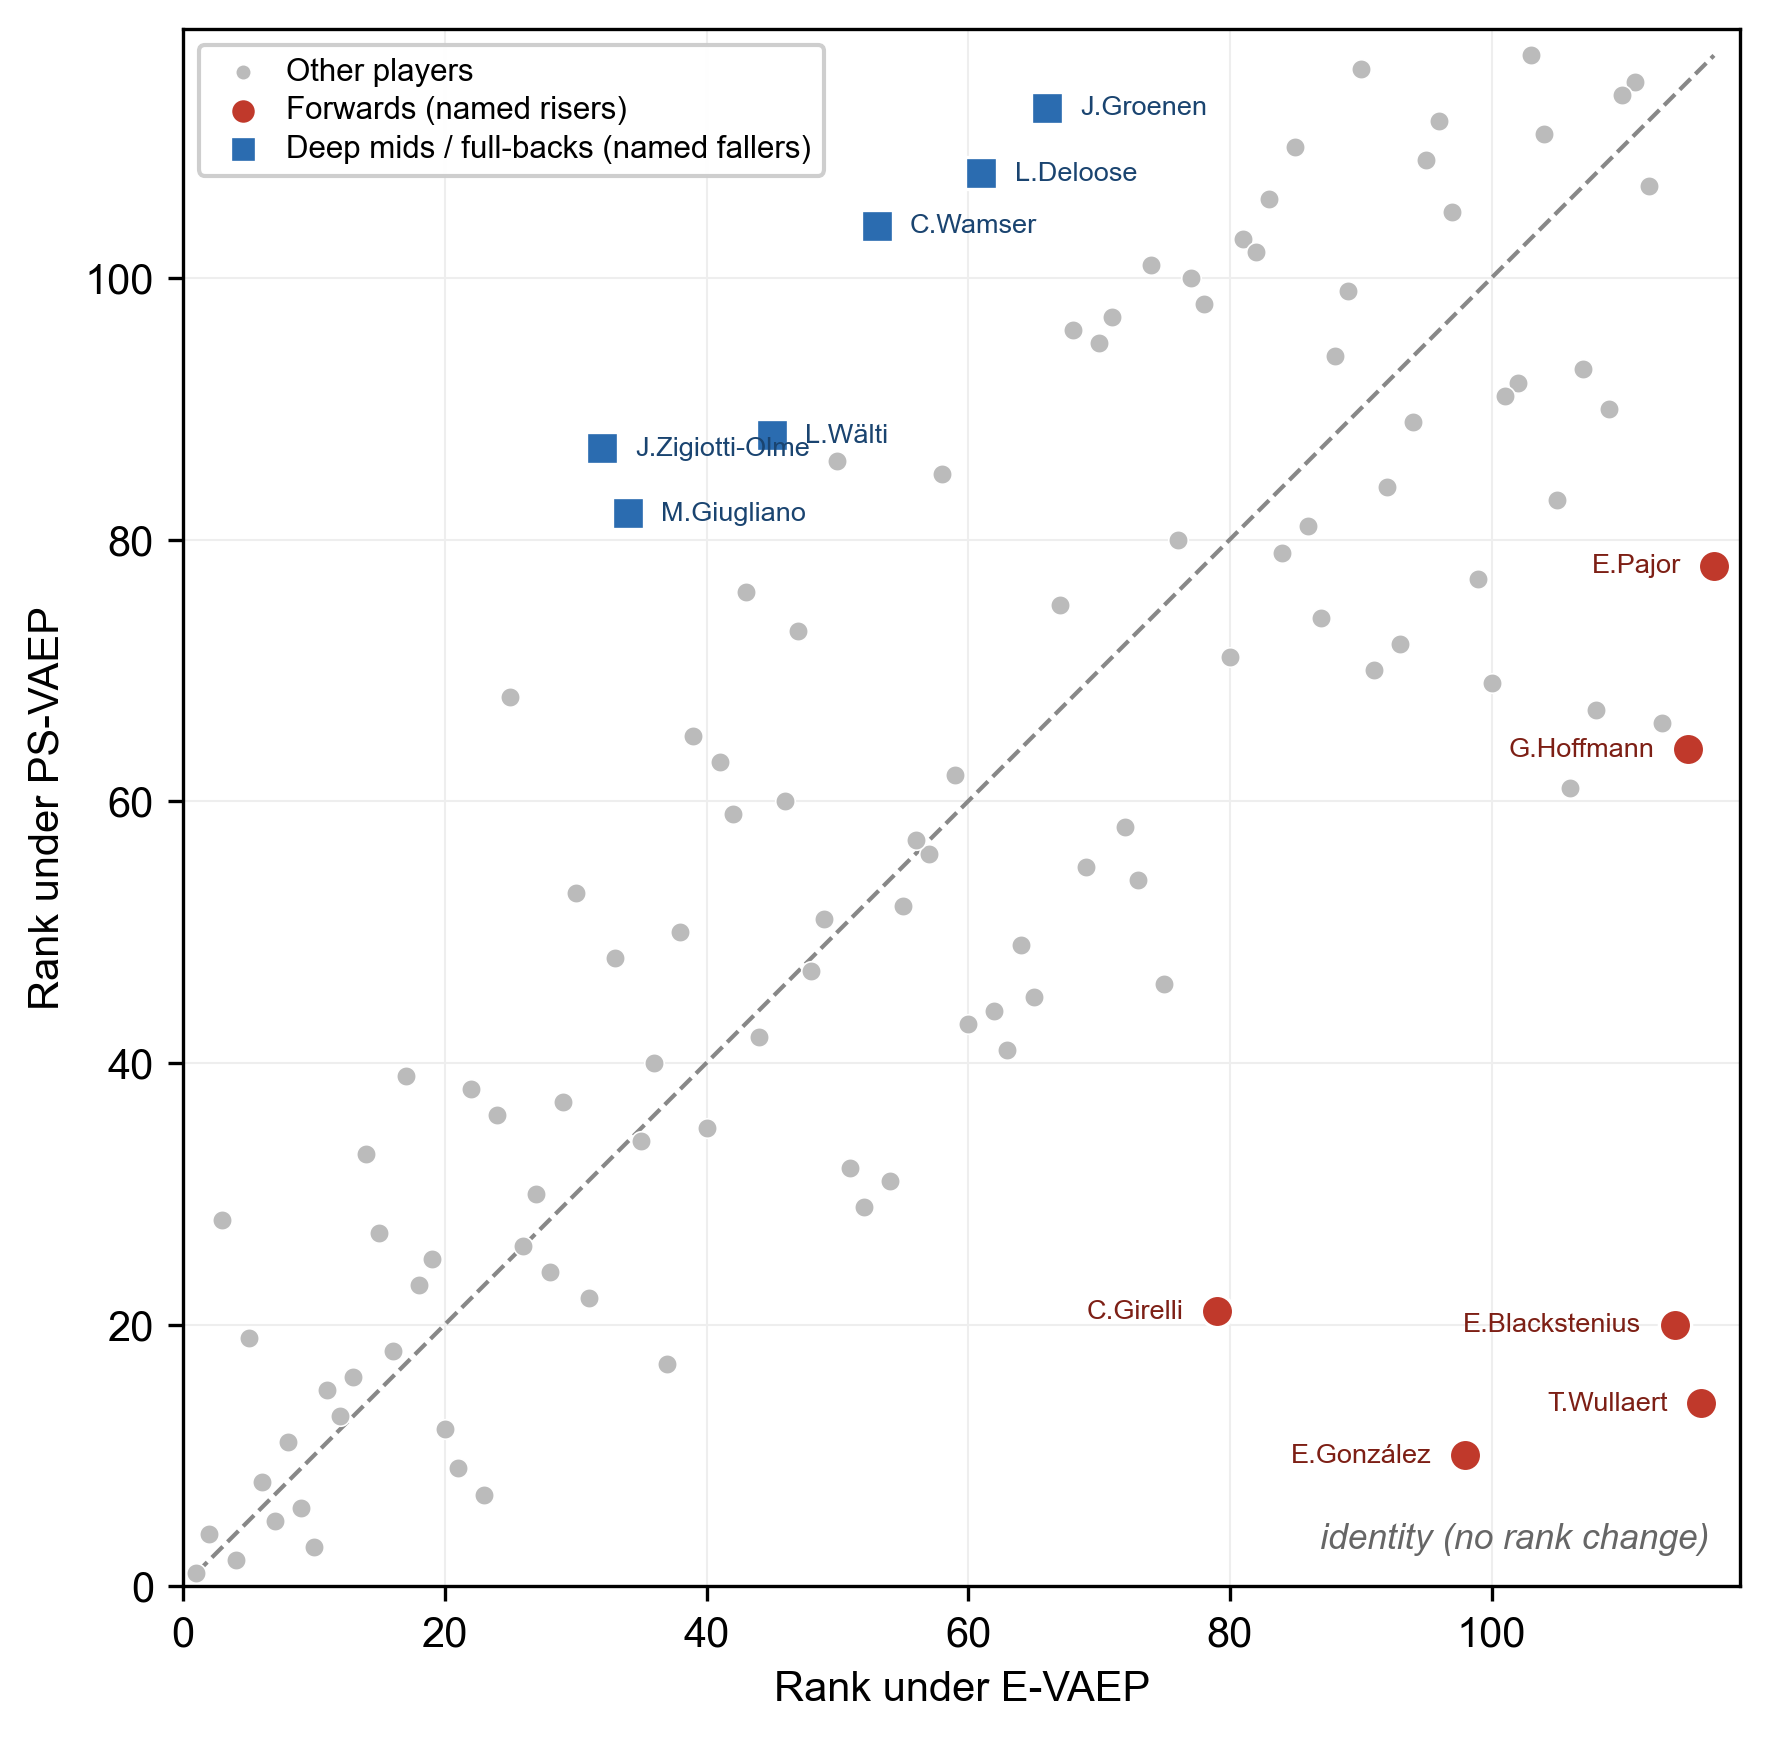
\includegraphics[width=\linewidth]{figures/figure_2.png}
\vspace{0.2em}
\footnotesize \textbf{(a)} Rank under E-VAEP versus   PS-VAEP
\end{minipage}
\hfill
\begin{minipage}[t]{0.40\textwidth}
\centering
\includegraphics[width=\linewidth]{figures/article_maanum}
\vspace{0.2em}
\footnotesize \textbf{(b)} Maanum take-on freeze frame.
\end{minipage}
\caption{Two views of PS-VAEP revaluation. Panel (a) shows player-level rank changes after adding spatial features; points below the diagonal rise under PS-VAEP. Panel (b) shows an action-level case in which dense local pressure leads PS-VAEP to assign a higher value than E-VAEP and P-VAEP.}
\label{fig:revaluation}
\end{figure}
Individual rank changes carry substantial uncertainty: of the 117 qualifying players, only 32 have a rank change whose bootstrap interval excludes zero. Among those, the largest upward shifts are Severini ($+50$ ranks), Hoffmann ($+41$), Pajor ($+35$), Bacha ($+34$), James ($+31$) and Naalsund ($+29$); the largest downward shifts are Zigiotti-Olme ($-52$), Groenen ($-52$), W\"alti ($-42$) and Deloose ($-41$). The upward group mixes central midfielders, forwards and a full-back, and the downward group is dominated by deep-lying midfielders. We therefore do not claim that the redistribution follows positional lines in any simple way; the pattern visible in panel (a) of Fig.~\ref{fig:revaluation} is a broad reordering rather than a clean positional rotation.

\subsection{Where the Added Context Matters}
\label{sec:strata}
To test what drives the reordering, we decompose the per-action change $\Delta = V_{\mathrm{PS}}(a) - V_{\mathrm{P}}(a)$ across defensive density, distance to the nearest opponent, pitch zone, action type and outcome, with match-level bootstrap intervals on each stratum mean.

The evidence supports a congestion mechanism and not a pressure mechanism. Actions with three or more visible opponents within 5~m --- 5.2\% of the evaluation set --- are the only stratum with a robustly positive mean change ($+0.0023$, CI $[+0.0005, +0.0039]$); every other density level shifts slightly negative. By contrast, distance to the nearest opponent produces no gradient at all ($-0.0015$, $-0.0018$, $-0.0014$ and $-0.0013$ across $<2$, $2$--$5$, $5$--$10$ and $>10$~m), and neither does pitch zone: penalty-area actions shift by $-0.0017$ with an interval spanning zero, against $-0.0014$ in the middle third. By action type, passes shift down slightly ($-0.0026$) while carries are essentially unchanged ($-0.0001$); the largest robust negative shifts fall on throw-ins ($-0.0105$) and goalkeeper claims ($-0.0159$) rather than on open-play progression.

We also test whether broadcast coverage explains the redistribution, since freeze frames record only players visible in the camera view and coverage varies systematically across the pitch. Coverage does vary by zone, from 14.4 visible players on average in the middle third to 12.2 in the penalty area, but the Spearman correlation between the number of visible players and $\Delta$ is $0.019$ overall and $0.065$ within the penalty area. Partial visibility is therefore not a plausible driver of the observed revaluation.

\paragraph{An illustration.}
Panel (b) of Fig.~\ref{fig:revaluation} shows one action in the congestion stratum described above: a take-on by Frida Maanum against Iceland, centrally in the penalty area, with four opponents within 5 m and four between the ball and the goal. E-VAEP and P-VAEP assign negative values ($-0.196$ and $-0.200$) whereas PS-VAEP assigns $+0.204$. Maanum rises from 10th to 3rd in total VAEP per 90, a shift of $+7$ ranks whose bootstrap interval excludes zero. The example illustrates the mechanism established above; on its own it would not establish one.
\section{Discussion and Limitations}
\label{sec:limitations}
The results separate two effects that are often conflated in action valuation. Tactical phase context improves probability estimation on the conceding head, and this is the only difference anywhere in our ablation that survives match-level resampling. Freeze-frame spatial context does not improve aggregate prediction at this data scale --- its one robust effect on predictive quality is a small degradation of scoring discrimination --- yet it reorders the player ranking to a degree the phase layer does not, from $\rho = 0.97$ to $\rho = 0.83$ against the event-only baseline.

That the two layers separate this cleanly is the paper's main observation. It also suggests that contextual valuation models should not be assessed only by ROC-AUC or log loss: a model can leave aggregate probability quality untouched while reallocating credit across players and situations. In our setting PS-VAEP is a revaluation model, not a predictively superior one.

We are deliberately neutral about whether this reallocation is an improvement. Reduced credit for progression in open space is not evidence of a correction, and may well be a defect: our models value on-ball actions only, so where the space for a progressive pass was created by preceding off-ball movement, PS-VAEP's lower valuation reflects the model's blind spot rather than better judgement. Adjudicating the direction of the redistribution requires independent expert assessment, which we have not performed.

The evidence for the mechanism is likewise partial. The stratified analysis supports congestion --- actions with three or more opponents within 5~m gain value robustly --- but not pressure, since distance to the nearest opponent produces no gradient, and not location, since pitch zone produces none either. A narrower claim than the one we set out to test is what the data support.

Several limitations remain. The evaluation is a single held-out women's tournament, and one tournament is a thin basis for the wide intervals we report. Freeze frames observe only players visible in the broadcast view; we show that coverage does not explain the redistribution, but coverage still bounds what the spatial features can encode. The phase taxonomy is rule-based and will mislabel edge cases. Pooled training uses more data than either single-domain strategy, so our transfer results do not separate cross-domain complementarity from sample size; a size-matched comparison and learning curves in the number of training matches would settle this and are the most useful next step. Finally, we compare against event-only and phase-only baselines rather than against learned freeze-frame representations such as those used for pass valuation~\cite{robberechts2023unxpass}; a direct comparison would better position the interpretable-feature route we take here.
\paragraph{Disclosure of Interests.}
The authors declare no competing interests.
% ---- Bibliography ----
\bibliographystyle{splncs04}
\bibliography{women_vaep_references}
\end{document}
